\documentclass{article}

\usepackage{tikz}
\usetikzlibrary{external,shapes,calc,math,patterns,arrows,positioning,fadings}
\tikzexternalize[optimize=false]

\tikzstyle{node}=[circle, draw=black, minimum size=25pt, line width=1, inner sep= 5pt]
\tikzstyle{nodel}=[circle, draw=black, minimum size=15pt, line width=1, inner sep= 0pt]
\tikzstyle{nodem}=[circle, draw=black, minimum size=10pt, line width=1, inner sep= 0pt]
\tikzstyle{tnode}=[nodel, minimum size=0.8 cm, fill=white]
\tikzstyle{node1}=[circle, draw=black, minimum size=15pt, line width=1, inner sep= 2pt]
\tikzstyle{node2}=[circle, draw=black, minimum size=8pt, line width=1, inner sep= 0pt, fill=white!70!black]
\tikzstyle{l1}=[line width=1]
\tikzfading[name=fade right, left color=transparent!0, right color=transparent!100]
\tikzstyle{odd}=[node1, dashed, pattern=dots, pattern color=mred!75!white]
\tikzstyle{even}=[node1, pattern=dots, pattern color=mblue!75!white]
\tikzstyle{lodd}=[odd, pattern = crosshatch dots]
\tikzstyle{leven}=[even, pattern = crosshatch dots]
\tikzstyle{enset}=[node1, thick, double, font=\footnotesize]
\tikzstyle{onset}=[node1, thick, densely dashed, double, font=\footnotesize]
\tikzstyle{subtree}=[node1, opacity=0.3,dotted, font=\footnotesize]
\tikzstyle{undef}=[node1, dotted, pattern=dots, pattern color=black!25!white]

\usepackage{xcolor}
\definecolor{mblue}{HTML}{1F77B4}
\definecolor{morange}{HTML}{FF7F0E}
\definecolor{mgreen}{HTML}{2CA02C}
\definecolor{mred}{HTML}{D62728}
\definecolor{mpurple}{HTML}{9467BD}
\definecolor{mbrown}{HTML}{8C564B}
\definecolor{mpink}{HTML}{E377C2}
\definecolor{mgrey}{HTML}{7F7F7F}
\definecolor{mlime}{HTML}{BCBD22}
\definecolor{mcyan}{HTML}{17BECF}

% Set new commands
\newcommand{\codeword}[1]{\texttt{\textcolor{MidnightBlue}{#1}}}
%\newcommand{\codefunc}[1]{\texttt{\textcolor{OliveGreen}{#1}}}
\let\oldemptyset\emptyset
\let\emptyset\varnothing
\newcommand{\codefunc}[1]{\texttt{#1}}
\newcommand{\m}[1]{\mathcal{#1}}
\newcommand{\n}[1]{\mathscr{#1}}
\newcommand{\bound}{\mathscr{B}}
\newcommand{\akker}{\mathscr{A}}
\newcommand{\nset}{\mathcal{N}}
\newcommand{\vset}{\mathcal{V}}
\newcommand{\pre}[1]{ {}^{#1} }
\newcommand{\ceil}[1]{{\left \lceil #1 \right \rceil }}
\newcommand{\floor}[1]{{\left \lfloor #1 \right \rfloor }}


\begin{document}
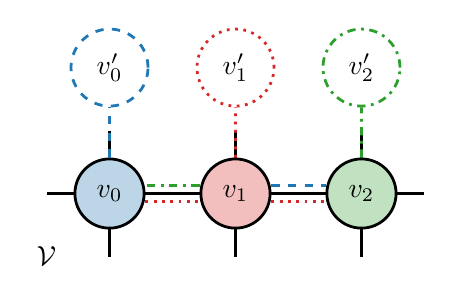
\begin{tikzpicture}[scale=0.8]

    \node at (-1, -1) {$\mathcal{V}$};
    \draw[l1] (0, 0) -- (4,0);
    \draw[l1] (-1,0) -- (5,0);
    \draw[l1] (0,1) -- (0,-1);
    \draw[l1] (2,1) -- (2,-1);
    \draw[l1] (4,1) -- (4,-1);
    \node[node, fill=white!70!mblue, text opacity=1] at (0,0) (1) {$v_0$};
    \node[node, draw=mblue, dashed] at (0,2) (2) {$v_0'$};
    \node[node, fill=white!70!mred, text opacity=1] at (2,0) (3){$v_1$};
    \node[node, draw=mred,dotted] at (2,2) (4) {$v_1'$};
    \node[node, fill=white!70!mgreen, text opacity=1] at (4,0) (5) {$v_2$};
    \node[node, draw=mgreen, dashdotted] at (4,2) (6) {$v_2'$};

    \draw[l1, dashed, mblue] (1) -- (2);
    \draw[l1, dashed, mblue, transform canvas={yshift=3pt}] (3) -- (5);
    \draw[l1, dotted, mred] (3) -- (4);
    \draw[l1, dotted, mred, transform canvas={yshift=-3pt}] (1) -- (3) -- (5);
    \draw[l1, dashdotted, mgreen] (5) -- (6);
    \draw[l1, dashdotted, mgreen, transform canvas={yshift=3pt}] (3) -- (1);

\end{tikzpicture}

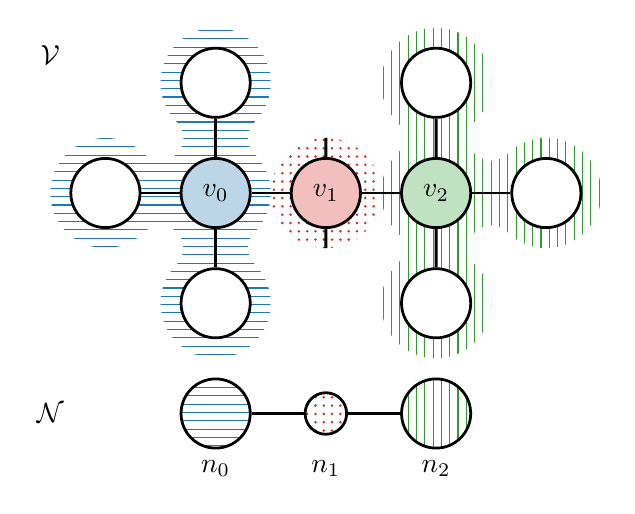
\begin{tikzpicture}[scale=0.7]
    \path[pattern=horizontal lines, pattern color=mblue] (0,3) arc (90:225:1) arc (45:-135:.4142) arc (45:315:1) arc (135:-45:.4142) arc (135:405:1) arc (225:135:.4142) arc (-45:45:1) arc (225:135:.4142) arc (-45:90:1) -- cycle;

    \begin{scope}[shift={(4,0)}, xscale=-1]
        \path[pattern=vertical lines, pattern color=mgreen] (0,3) arc (90:225:1) arc (45:-135:.4142) arc (45:315:1) arc (135:-45:.4142) arc (135:405:1) arc (225:135:.4142) arc (-45:45:1) arc (225:135:.4142) arc (-45:90:1) -- cycle;
    \end{scope}
    \path[pattern=dots , pattern color=mred] (2,1) arc (90:450:1);

    \node[node, fill=white!70!mblue] at (0,0) (0) {$v_0$};
    \node[node, fill=white!70!mred] at (2,0) (1) {$v_1$};
    \node[node, fill=white!70!mgreen] at (4,0) (5) {$v_2$};
    \node[node, fill=white] at (-2,0) (2) {};
    \node[node, fill=white] at (0,2) (3) {};
    \node[node, fill=white] at (0,-2) (4) {};
    \node[node, fill=white] at (6,0) (6) {};
    \node[node, fill=white] at (4,2) (7) {};
    \node[node, fill=white] at (4,-2) (8) {};


    \draw[l1] (6) -- (5) -- (1) -- (0) -- (3);
    \draw[l1] (2) -- (0) -- (4);
    \draw[l1] (7) -- (5) -- (8);
    \draw[l1] (2, 1) -- (1) -- (2,-1);
    \node at (-3, 2.5) {$\mathcal{V}$};

    \begin{scope}[shift={(0, -4)}]
        \node at (-3, 0) {$\mathcal{N}$}; 
        \node[node, pattern=horizontal lines, pattern color=mblue] at (0,0) (d) {};
        \node[nodel, pattern=dots , pattern color=mred] at (2,0) (e) {};
        \node[node, pattern=vertical lines, pattern color=mgreen] at (4,0) (f) {};
        \node at (0,-1) {$n_0$};
        \node at (2,-1) {$n_1$};
        \node at (4,-1) {$n_2$};
        \draw[l1] (d) -- (e) -- (f);
    \end{scope}


\end{tikzpicture}

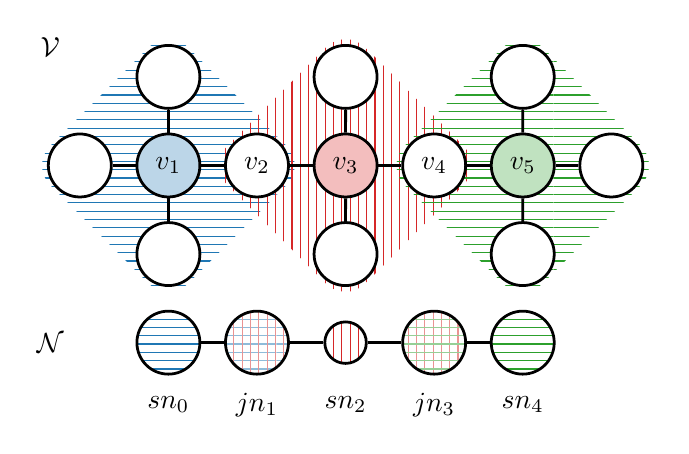
\begin{tikzpicture}[scale=0.75]
    \node at (-3, 2) {$\mathcal{V}$};
    \node at (-3, -3) {$\mathcal{N}$}; 


    \begin{scope}[shift={(-1, 0)}, scale=1.5]
        \node at (0,0) (0) {}; \node at (2,0) (1) {}; \node at (4,0) (2) {};        
        \path[pattern=horizontal lines, pattern color=mblue, rounded corners=10pt, rotate around={45:(0)}] (-1.1,-1.1) rectangle (1.1,1.1);
        \path[pattern=vertical lines, pattern color=mred, rounded corners=10pt, rotate around={45:(1)}] (0.9,-1.1) rectangle (3.1,1.1);
        \path[pattern=horizontal lines, pattern color=mgreen, rounded corners=10pt, rotate around={45:(2)}] (2.9,-1.1) rectangle (5.1,1.1);
    
        \node[tnode, fill=white!70!mblue] at (0) (v0) {$v_1$};
        \node[tnode] at (-1,0) (v0l) {};
        \node[tnode] at (0,1) (v0u) {};
        \node[tnode] at (0,-1) (v0d) {};
    
        \node[tnode, fill=white!70!mred] at (1) (v1) {$v_3$};
        \node[tnode] at (1,0) (v1l) {$v_{2}$};
        \node[tnode] at (2,1) (v1u) {};
        \node[tnode] at (2,-1) (v1d) {};
    
        \node[tnode, fill=white!70!mgreen] at (2) (v2) {$v_5$};
        \node[tnode] at (3,0) (v2l) {$v_{4}$};
        \node[tnode] at (5,0) (v2r) {};
        \node[tnode] at (4,1) (v2u) {};
        \node[tnode] at (4,-1) (v2d) {};
    
        \draw[l1] (v0l) -- (v0) -- (v1l) -- (v1) -- (v2l) -- (v2) -- (v2r);
        \draw[l1] (v0u) -- (v0) -- (v0d);
        \draw[l1] (v1u) -- (v1) -- (v1d);
        \draw[l1] (v2u) -- (v2) -- (v2d);
    \end{scope}

    \begin{scope}[shift={(-1, -3)}, scale=1.5]
        \node[tnode, pattern=horizontal lines, pattern color=mblue] at (0,0) (n0) {};
        \node[tnode, pattern=horizontal lines, pattern color=mblue!50!white, line width=0] at (1,0) {};
        \node[tnode, pattern=vertical lines,   pattern color=mred!50!white] at (1,0) (j01) {};
        \node[nodel, pattern=vertical lines , pattern color=mred] at (2,0) (n1) {};
        \node[tnode, pattern=vertical lines,   pattern color=mred!50!white, line width=0] at (3,0) {};
        \node[tnode, pattern=horizontal lines, pattern color=mgreen!50!white] at (3,0) (j12) {};
        \node[tnode, pattern=horizontal lines, pattern color=mgreen] at (4,0) (n2) {};
        \node at (0,-.7) {$sn_0$};
        \node at (1,-.7) {$jn_{1}$};
        \node at (2,-.7) {$sn_2$};
        \node at (3,-.7) {$jn_{3}$};
        \node at (4,-.7) {$sn_4$};
        \draw[l1] (n0) -- (j01) -- (n1) -- (j12) -- (n2);
    \end{scope}
\end{tikzpicture}

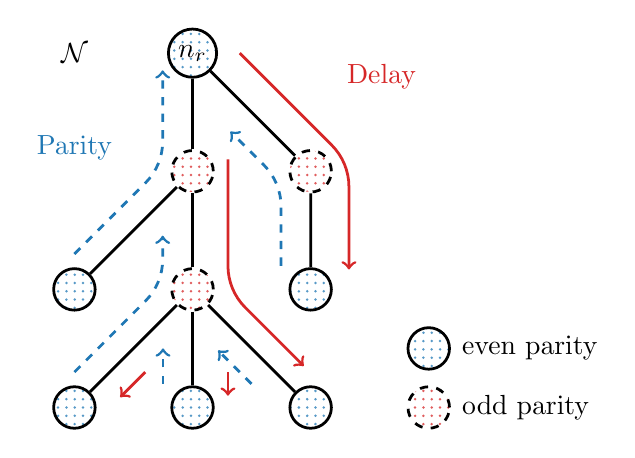
\begin{tikzpicture}[x=1.5cm,y=1.5cm]
    \node[node1,even] (a) at (1, 3) {$n_r$};
    \node[node1,odd]  (b) at (1, 2) {};
    \node[node1,odd]  (c) at (1, 1) {};
    \node[node1,even] (d) at (1, 0) {};
    \node[node1,even] (e) at (0, 1) {};
    \node[node1,even] (f) at (0, 0) {};
    \node[node1,odd]  (g) at (2, 2) {};
    \node[node1,even] (h) at (2, 1) {};
    \node[node1,even] (i) at (2, 0) {};
    \draw[l1] (a) -- (b) -- (c) -- (d);
    \draw[l1] (b) -- (e);
    \draw[l1] (c) -- (f);
    \draw[l1] (c) -- (i);
    \draw[l1] (a) -- (g) -- (h);

    \draw[l1, ->, dashed, color=mblue] (0, 1.3) -- +(45:0.85) arc (-45:0:.5) -- +(90:.6);
    \draw[l1, ->, dashed, color=mblue] (0, 0.3) -- +(45:0.85) arc (-45:0:.5) -- +(90:.2);
    \draw[l1, ->, dashed, color=mblue] (0.75,0.2) -- +(90:.3);
    \draw[l1, ->, dashed, color=mblue] (1.5,0.2) -- +(135:.4);
    \draw[l1, ->, dashed, color=mblue] (1.75,1.2) -- +(90:0.5) arc (0:45:.5) -- +(135:0.4);
    \draw[l1, ->, color=mred] (1.4, 3) -- +(-45:1.1) arc (45:0:0.5) -- +(-90:0.7);
    \draw[l1, ->, color=mred] (1.3, 2.1) -- +(-90:0.9) arc (180:225:.5) -- +(-45:0.7);
    \draw[l1, ->, color=mred] (0.6, 0.3) -- +(225:.3);
    \draw[l1, ->, color=mred] (1.3, 0.3) -- +(-90:.2);
    \node[text=mblue] at (0,2.2) {Parity};
    \node[text=mred] at (2.6,2.8) {Delay};
    \node at (0,3) {$\mathcal{N}$};

    \path (3,.5) node[node1, even]{} -- +(.2,0) node[anchor=west] {even parity}; 
    \path (3,0) node[node1, odd]{} -- +(.2,0) node[anchor=west] {odd parity}; 
\end{tikzpicture}

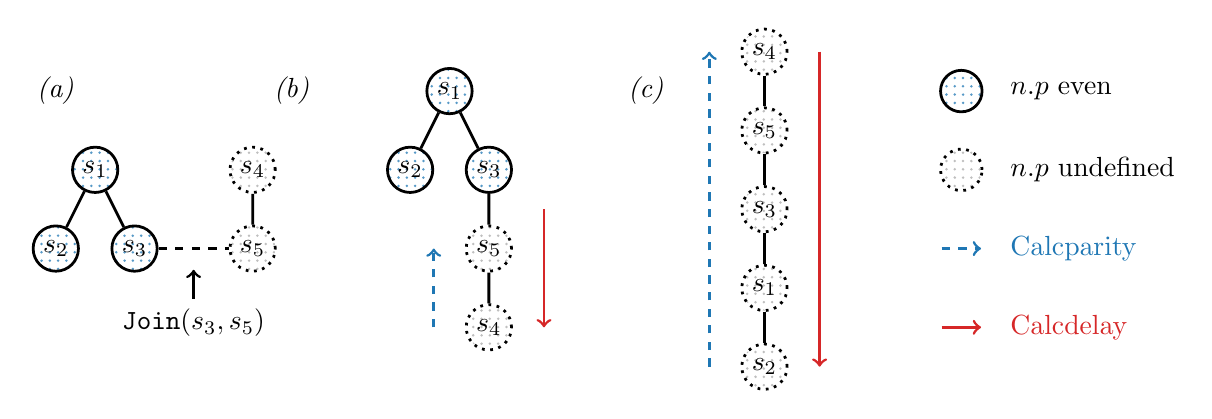
\begin{tikzpicture}[on grid]
    \node (o1) [even] at (1.5, 1) {$s_1$};
    \node (o2) [even] at (1, 0) {$s_2$};
    \node (o3) [even] at (2, 0) {$s_3$};
    \node (e4) [undef] at (3.5,1) {$s_4$};
    \node (e5) [undef] at (3.5,0) {$s_5$};
    \draw[l1] (o2) -- (o1) -- (o3) (e4) -- (e5);
    \draw[l1, dashed] (o3) -- (e5) node[midway,below] (a) {};
    \draw[l1, <-] (a) -- ++(0,-.5) node[below] {$\codefunc{Join}(s_3, s_5)$};
  
    \begin{scope}[shift={(4.5,1)}]
    \node (o1) [even] at (1.5, 1) {$s_1$};
    \node (o2) [even] at (1, 0) {$s_2$};
    \node (o3) [even] at (2, 0) {$s_3$};
    \node (e4) [undef] at (2,-2) {$s_4$};
    \node (e5) [undef] at (2,-1) {$s_5$};
    \draw[l1] (o2) -- (o1) -- (o3) -- (e5) -- (e4);
    \draw[l1, ->, dashed, color=mblue] (e4) ++(-.7,0) -- + (0,1);
    \draw[l1, ->, color=mred] (o3) ++(.7,-.5) -- +(0,-1.5);
    \end{scope}
  
    \begin{scope}[shift={(9,1.5)}]
    \node (o1) [undef] at (1, -2) {$s_1$};
    \node (o2) [undef] at (1, -3) {$s_2$};
    \node (o3) [undef] at (1, -1) {$s_3$};
    \node (e4) [undef] at (1,1) {$s_4$};
    \node (e5) [undef] at (1,0) {$s_5$};
    \draw[l1] (o2) -- (o1) -- (o3) -- (e5) -- (e4);
    \draw[l1, ->, dashed, color=mblue] (o2) ++(-.7,0) -- +(0,4);
    \draw[l1, ->, color=mred] (e4) ++(.7,0) -- +(0,-4);
    \end{scope}
  
    \node at (1,2) {\emph{(a)}};
    \node at (4,2) {\emph{(b)}};
    \node at (8.5,2) {\emph{(c)}};
    \path (12.5, 2) node[even] {} -- +(.5,0) node[anchor=west]{$n.p$ even};
    \path (12.5, 1) node[undef] {} -- +(.5,0) node[anchor=west]{$n.p$ undefined};
    \draw[l1, ->, color=mred] (12.25, -1) -- ++(0.5,0);
    \node[color=mred, anchor=west] at (13,-1) {Calcdelay};
    \draw[l1, ->, color=mblue, dashed] (12.25, 0) -- ++(0.5,0);
    \node[color=mblue, anchor=west] at (13,0) {Calcparity};
\end{tikzpicture}

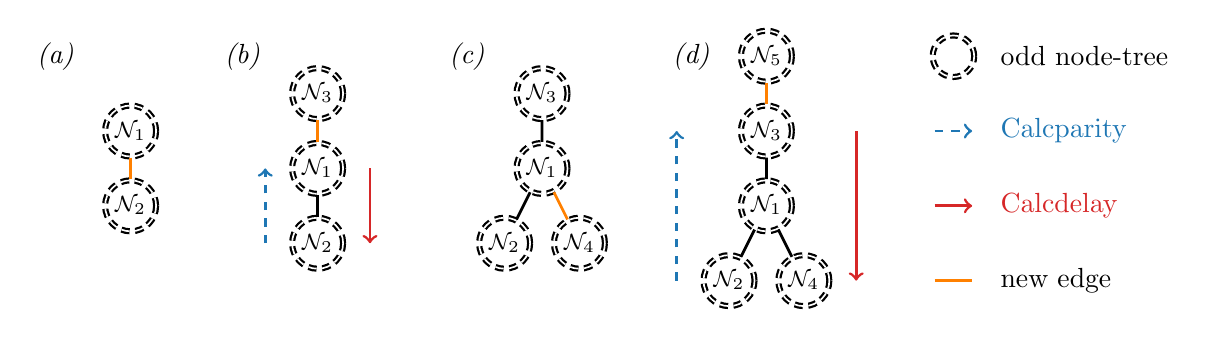
\begin{tikzpicture}[scale=0.95]
    \node (n1) [onset] at (0,0) {$\mathcal{N}_1$};
    \node (n2) [onset] at (0,-1) {$\mathcal{N}_2$};
    \draw[l1, color=orange] (n1) -- (n2);

    \begin{scope}[shift={(2.5,-.5)}]
    \node (n3) [onset] at (0,1) {$\mathcal{N}_3$};
    \node (n1) [onset] at (0,0) {$\mathcal{N}_1$};
    \node (n2) [onset] at (0,-1) {$\mathcal{N}_2$};
    \draw[l1, color=orange] (n3) -- (n1); \draw[l1] (n1) -- (n2);
    \draw[l1, ->, dashed, color=mblue] (n2) ++(-.7,0) -- +(0,1);
    \draw[l1, ->, color=mred] (n1) ++(.7,0) -- +(0,-1);
    \end{scope}

    \begin{scope}[shift={(5.5,-.5)}]
    \node (n3) [onset] at (0,1) {$\mathcal{N}_3$};
    \node (n1) [onset] at (0,0) {$\mathcal{N}_1$};
    \node (n2) [onset] at (-.5,-1) {$\mathcal{N}_2$};
    \node (n4) [onset] at (.5,-1) {$\mathcal{N}_4$};
    \draw[l1, color=orange] (n1) -- (n4); \draw[l1] (n3) -- (n1) -- (n2);
    \end{scope}

    \begin{scope}[shift={(8.5,-1)}]
    \node (n5) [onset] at (0,2) {$\mathcal{N}_5$};
    \node (n3) [onset] at (0,1) {$\mathcal{N}_3$};
    \node (n1) [onset] at (0,0) {$\mathcal{N}_1$};
    \node (n2) [onset] at (-.5,-1) {$\mathcal{N}_2$};
    \node (n4) [onset] at (.5,-1) {$\mathcal{N}_4$};
    \draw[l1, color=orange] (n3) -- (n5); \draw[l1] (n3) -- (n1) -- (n2) (n1) -- (n4);
    \draw[l1, ->, dashed, color=mblue] (n2) ++(-.7,0) -- +(0,2);
    \draw[l1, ->, color=mred] (n3) ++(1.2,0) -- +(0,-2);
    \end{scope}

    \node at (-1, 1) {\emph{(a)}};
    \node at (1.5, 1) {\emph{(b)}};
    \node at (4.5, 1) {\emph{(c)}};
    \node at (7.5, 1) {\emph{(d)}};

    \begin{scope}[shift={(11,1)}]
        \path (0,0)node[onset]{} -- +(.5,0)node[anchor=west]{odd node-tree};
        \draw[l1, ->, color=mred] (-.25, -2) -- ++(0.5,0);
        \node[color=mred, anchor=west] at (.5,-2) {Calcdelay};
        \draw[l1, ->, color=mblue, dashed] (-.25, -1) -- ++(0.5,0);
        \draw[l1, color=orange] (-.25, -3) -- ++(0.5,0);
        \node[color=mblue, anchor=west] at (.5,-1) {Calcparity};
        \node[anchor=west] at (.5,-3) {new edge};
    \end{scope}
\end{tikzpicture}

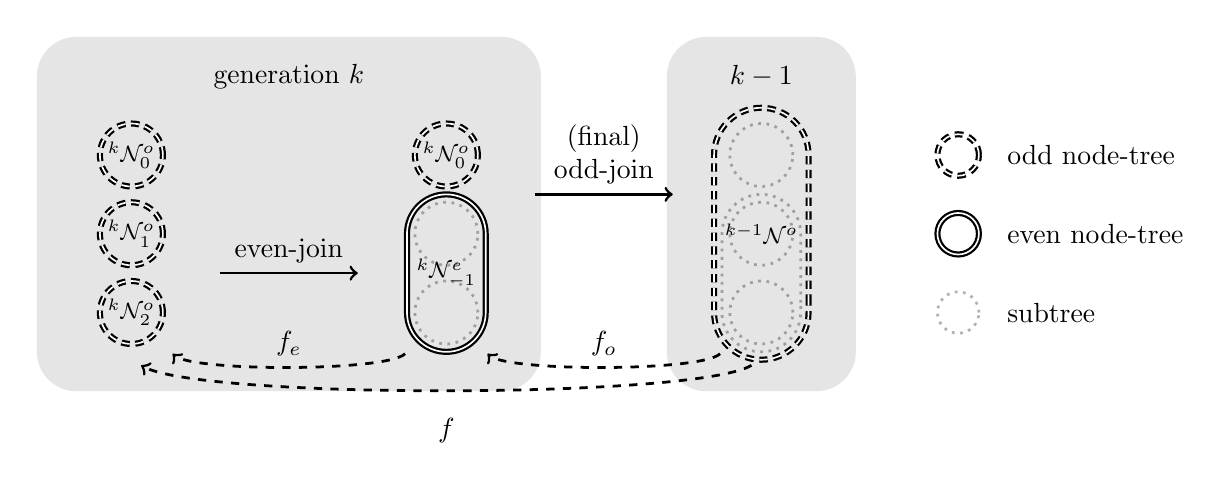
\begin{tikzpicture}[node distance=1cm, on grid]

    \node (a) at (0,0) {};
    \node (b) [right = 4cm of a] {};
    \node (c) [right = 4cm of b] {};
    \node (d) [right = 3cm of c] {};

    \node (b1l) [below left = 1cm and 1.2cm of a] {};
    \node (b1r) [above right = 3.5cm and 1.2cm of b] {};
    \path[fill=black!10!white, rounded corners=0.5cm] (b1l) rectangle (b1r);
    \node (b1t) at ($(a)!0.5!(b)$) {}; \node [above=3cm of b1t] {generation $k$};
    \node (b2l) [below left = 1cm and 1.2cm of c] {};
    \node (b2r) [above right = 3.5cm and 1.2cm of c] {};
    \path[fill=black!10!white, rounded corners=0.5cm] (b2l) rectangle (b2r);
    \node [above=3cm of c] {$k-1$};

    \begin{scope}[shift={(10.5,0)}]
      \path (0,2) node[onset]{} -- +(.5,0)node[anchor=west]{odd node-tree};
      \path (0,1) node[enset]{} -- +(.5,0)node[anchor=west]{even node-tree};
      \path (0,0) node[subtree]{} -- +(.5,0)node[anchor=west]{subtree};
    \end{scope}

    \node (a0) [above = 0 cm of a] {\footnotesize $\pre{k}\mathcal{N}^o_2$};
    \node (a1) [above = 1 cm of a] {\footnotesize $\pre{k}\mathcal{N}^o_1$};
    \node (a2) [above = 2 cm of a] {\footnotesize $\pre{k}\mathcal{N}^o_0$};
    \draw[onset] (a0) circle[radius=.4cm];
    \draw[onset] (a1) circle[radius=.4cm];
    \draw[onset] (a2) circle[radius=.4cm];

    \foreach \i in {0,1,2}{
        \node (b\i) [above = \i cm of b] {};
    }
    \node at (b2) {\footnotesize $\pre{k}\mathcal{N}^o_0$};
    \node at ($(b0)!0.5!(b1)$) {\footnotesize $\pre{k}\mathcal{N}^e_{-1}$};
    \draw[onset] (b2) circle[radius=0.4cm];
    \draw[subtree] (b1) circle[radius=.4cm];
    \draw[subtree] (b0) circle[radius=.4cm];
    \node[right = 0.5cm of b] (bc) {};
    \draw[enset] (bc) -- +(0, 1) arc (0:180:0.5) -- +(0, -1) arc (180:360:0.5) -- cycle;

    \foreach \i in {0,1,2}{
      \node (c\i) [above =\i cm of c] {};
      \draw[subtree] (c\i) circle[radius=.4cm];
    }
    \node[right = 0.5cm of c] (cc1) {}; \node[right = 0.6cm of c] (cc2) {};
    \draw[subtree] (cc1) -- +(0, 1) arc (0:180:0.5) -- +(0, -1) arc (180:360:0.5) -- cycle;
    \draw[onset] (cc2) -- +(0, 2) arc (0:180:0.6) -- +(0, -2) arc (180:360:0.6) -- cycle;
    \node at (c1) {\footnotesize $\pre{k-1}\mathcal{N}^o$};

    \node (f1a) [below left = 0.4cm and 0.4cm of c] {}; \node (f1b) [below right = 0.4cm and 0.4cm of b] {};
    \node (f2a) [below left = 0.4cm and 0.4cm of b] {}; \node (f2b) [below right = 0.4cm and 0.4cm of a] {};
    \node (fa) [below = 0.6cm of c] {}; \node (fb) [below = 0.6cm of a] {};
    \draw[l1, ->, dashed] (f1a) .. controls +(225:0.5cm) and +(315:0.5cm) .. (f1b);
    \draw[l1, ->, dashed] (f2a) .. controls +(225:0.5cm) and +(315:0.5cm) .. (f2b);
    \draw[l1, ->, dashed] (fa)  .. controls +(210:1cm) and +(330:1cm) .. (fb);

    \node (ca) at ($(c)!0.5!(a)$) {}; \node [below = 1.5cm of ca] {$f$};
    \node (cb) at ($(c)!0.5!(b)$) {}; \node [below = 0.4cm of cb] {$f_o$};
    \node [below = 0.4cm of b1t] {$f_e$};

    \node (u1lt) at ($(a0)!0.5!(a1)$) {}; \node(u1l) [right=1cm of u1lt] {};
    \node (u1rt) at ($(b0)!0.5!(b1)$) {}; \node(u1r) [left=1cm of u1rt] {};
    \node (u2lt) at ($(b1)!0.5!(b2)$) {}; \node(u2l) [right=1cm of u2lt] {};
    \node (u2rt) at ($(c1)!0.5!(c2)$) {}; \node(u2r) [left=1cm of u2rt] {};
    \draw[l1, ->] (u1l) -- (u1r) node[midway,above] {even-join};
    \draw[l1, ->] (u2l) -- (u2r) node[midway,above, text width = 2cm, align=center] {(final)\\odd-join};

\end{tikzpicture}
\end{document}